\documentclass[12pt, a4paper]{report}
\usepackage{graphicx}
\usepackage[export]{adjustbox}
\usepackage{listings}

\newenvironment{loggentry}[2]% date, heading
{\noindent\textbf{#2}\newline\{\marginnote{#1}\}\newline\\}{\vspace{1.0cm}}

\begin{document}
\begin{titlepage}
	\centering
	
\includegraphics[width=0.15\textwidth]{res/inf.png}\par\vspace{1cm}
	{\scshape\LARGE UFRGS - Instituto de Informatica \par}
	\vspace{1cm}
	{\scshape\Large Volunteer Project\par}
	\vspace{1.5cm}
	{\huge\bfseries Kelvinlets Video Deformation\par}
	\vspace{2cm}
	{\Large\itshape Guilherme Gomes Haetinger\par}
	\vfill
	supervised by\par
	Dr. Eduardo S. L. \textsc{Gastal}

	\vfill

% Bottom of the page
	{\large \today\par}
\end{titlepage}

\begin{figure}
	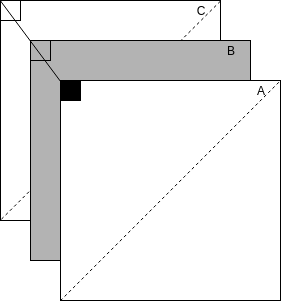
\includegraphics[scale=0.5, center]{./res/interpolationExample.png}
	\caption{3D Interpolation with Prism projection. (A) is the first grid involving the frame (B), and (C) is the second one.}
	\label{fig:newInterp}
\end{figure}

\begin{loggentry}{28-05-2019}{New Idea for 3D Interpolation}
	Based on the idea of interpolating 3D Cuboids on video frames, I wonder: are there other (better) ideas for this instead of Interpolating the tetrahedrons inside the prisms? One hypothesis is a prism projection on the video frames [\ref{fig:newInterp}].	

	The idea of establishing Scan Conversion on the Frame mesh based solely on line interpolation between the preprocessed grids seems really faster than the tetrahedron approach. Whereas we would process every point inside a bounding box delimited by the corners of every tetrahedron inside a Cuboid (6 volumes), we now process one pixel related to 2 others, which colors will interpolate, and scan convert the remaining pixels of the frame with the produced ones, as we would do in the KelvinletsImageGL code. I like to call this new method 2 step interpolation.  
\end{loggentry}

\begin{loggentry}{30-05-2019}{Elaborating Implementation for 2 step Interpolation}
		Having in mind the Professor's advice to use a \textit{bin sort} alike algorithm, the main goal is to set which lines collide with each of the frames. We do that by assigning each vertex from the frame having 2 points: one in each deformed frame. Based on that, we can establish the color and position of the vertices. Now, considering the order that the vertices must be processed, we should run them by the time axis, i.e. Interpolate the same pixel position for each frame before moving to another position.    
\end{loggentry}

\begin{loggentry}{(01 - 03)-06-2019}{Project Structure}
	Creating the projects structure is a challenge. Separating a OpenGL application in modules is somewhat difficult because of the fact that many functions depend on predeclared variables, which means I need many arguments for a specific function. Therefore, I will, firstly, separate the needed functionalities in main components. These components are:
	\begin{itemize}
		\item Main
											
			This module will only serve to process the user arguments set in \textit{argv} and to call the other methods with these arguments.
		
		\item VideoDeformator
									
			This module will be in charge of processing the arguments given by the \textit{Main} modules in order to execute the Kelvinlets \textit{grab} function in each vertex. It will produce a new set of vertex arrays for the ones in the video input (regularized vertices). This module will include the \textbf{glm} and the \textbf{glfw3} library, since it will depend on the data structures involving linear algebra as well as the ones defined for OpenGL visualization.

			\begin{itemize}
				\item[$\ast$] InterpolationFrame

					This data structure should hold every line in charge of interpolating each vertex of the frame.
				
				\item[$\ast$] Line

					This data structure should hold the information to interpolate a line in a given point in the time axis.

				\item[$\ast$] Deformation

					Abstraction of a deformation vector(initial position, final position and brush size).

				\item[$\ast$] KelvinletsTransformer

					Class that provides the execution of the Kelvinlets equation.
			
			\end{itemize}
		
		\item VideoVisualizer

			This module will be responsible for the video rendering, i.e. the communication of the program with the deformed  video data and the graphic card. To do this, we must use the OpenGL library, for which we will need the vertices positions and colors, as well as the order in which they will be accounted for the triangle mesh rendering in the \textbf{TRIANGLE\_STRIP} method. We are supposed to import, for these reasons, \textbf{glfw3} and \textbf{glew} for the data structures and graphic card communication functions.

	\end{itemize}

	For the sake of the project and organization, I also developed a \textbf{logger} for the application. This will make debugging much cleaner and easier. All I have to do to get specific output (errors, fatal errors, warnings and general debugging logs) is call the program in the following way:

\lstset{
  language=bash,
  basicstyle=\ttfamily
}

\begin{lstlisting}
  env KELVIN=FATAL|ERROR|WARNING|CORRECT|DEBUG ./kelvin
\end{lstlisting}

\end{loggentry}

\end{document}
